\section{Introduction}
Mobile software engineers have a finite amount of time and resources while working through the software development life cycle. How does an engineer decide where she should budget more time and resources to get the most return for her investment? Instrumentation within a hybrid mobile application can provide metrics based on user interaction. These metrics can be turned into actionable insights for the developer to better understand how users use the application. Based on these insights and understanding the developer can then focus on the popular aspects of the application and increase her return on investment. 

Hybrid mobile applications are applications which are written in web languages such as JavaScript, HTML 5, and CSS.  Unlike native applications which are written in a programming language specific to the mobile platform. Hybrid mobile applications are written once and distributed across multiple platforms. We talk more about hybrid mobile applications in the background section of the paper.

According to a survey by Java World, software engineers spend more than half of their time on tasks unrelated to software development \cite{JavaWorld}. The engineers are spending time on necessary tasks related to administration, waiting for code to build, and tests to execute. This is an interesting statistic and one that highlights how necessary effective resource management is. The survey also says that software engineers spend about 10\% of their time waiting for tests to complete. A developer who has insight and understands her users will be able to target key functionality. This targeted approach will allow the developer to maximize her time on areas of the application that are used the most. In addition, this approach will also enable to developer to write meaningful tests in areas of code that are most used. 

There really is not a good way in hybrid mobile application development to collect user interaction data at the function level. There are plenty of tools that are decent at collecting hardware statistics from mobile devices. We talk about a few of these tools in the related works section of the paper. There are also a couple of tools that offer some insight into user interaction but none that offer the fidelity of information that our framework provides. These tools are also discussed in the related work section of the paper.

It is hard to tell why there are not good ways of collecting hybrid mobile application metrics. First, we needed to see if developers cared about user metrics and identifying user behaviors. We also wanted to know if developers would like to be able to collect information on function usage and frequency. In order to solve this issue we conducted a developer survey. Based on this survey and the amount of interest we gathered from developer we decided it would be worthwhile to find a novel way to collect hybrid mobile application metrics.

In order to evaluate our research we came up with 3 criteria to evaluate against: 
\begin{enumerate}
\item Do developers want metrics that can produce insights into user behavior and feature usage?
\item Does the application we created identify user behaviors?
\item Does the application identify the frequency of functions that are used?
\end{enumerate}
Through this research we have contributed:
\begin{itemize}
\item An open source software project that allows researchers to stand up a web service where developers can push data, using a RESTful web service, to persistent storage utilizing relational databases or time series databases.
\item A novel Node framework that collects user interaction metrics and pushes the data to a web service for insight analysis.
\item A developer study where we surveyed a number of developers to  gauge the usefulness of collecting metrics using time-series analysis. 
\item Discussion of insights that could be gathered using our tool and approach
\end{itemize}

\section{Background}
Our research and framework are built around two emerging platforms. Throughout this paper we discuss mobile hybrid applications and time series analysis. 
\subsection{Mobile Hybrid Applications}
Hybrid mobile applications have taken the market by storm.  A few of the benefits of using hybrid mobile applications is the portability, cheaper origination costs, and faster speeds to market. Companies such as Facebook, Adobe, and Apache have released frameworks and platforms to foster the development of hybrid mobile applications. Companies such as Tesla, Facebook, Walmart, Instagram, Skype, and Airbnb to name a few are using JavaScript based applications ~\cite{react-native}. 
\subsection{Time Series Analysis}
Time series analysis is not a new idea in the world of analytics. Analysts on Wall Street have been using time-series analysis for decades to measure stock values. Time series analysis has begun to become more prominent in the world of software engineering because more and more tools are taking advantage of it. There are now databases created just to manage time series data. James Blackburn does a good job of explaining time series analysis, time series analysis is the collection of data at specific intervals over a period of time, with the purpose of identifying trends, cycles, and variances to aid in the forecasting of a future event. Data is any observed outcome that is measurable. Unlike in statistical sampling, in time series analysis, data must be measured over time at consistent intervals to identify patterns that form trends, cycles, and seasonal variances. Measurements at random intervals lose the ability to predict future events"\cite{timeseries}.

We use time series analysis in our research to identify user behavior trends as we collect user interaction metrics. The time series allow us to identify usage trends of functionality within the mobile application. 

\section{Needs Assessment}
We could see the usefulness of collecting metrics inside of hybrid mobile applications. We could also see the benefits of understanding user behavior inside of an application. What we did not know was whether other developers could see the value in such things. We realized that we needed to gather more information and get input from other sources. We put together 20 survey questions and asked developers at a local company what they thought. Based on the survey responses, which we talk about more in the developer survey section, we realized that we were not alone. Other developers understood the benefits of collecting such metrics. We set out then to create an application which would help developers collect metrics and identify user trends and behaviors, which we talk about in the the application section.

\section{The Application}
\begin{figure}  
\begin{center}  
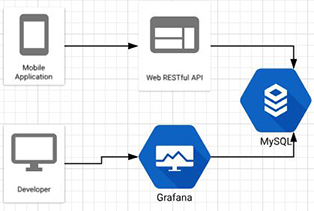
\includegraphics[]{arc2.JPG}  
\caption{\small \sl Architecture Example\label{fig:architecture_example}}  
\end{center}  
\end{figure}  

Based on the amount of interest we received from our developer survey, we set out to create an application which would allow us to collect metrics whioch provide insights into user behavior and function usage. Here is a high level overview of how the system works.

There are three core components to the tool that we developed. The first component is the Node middleware module. The second component is the web service which provides an API for the middleware to send data to. The last component is the metric analytics and visualization. This component offers developers a graphical user interface to interact with the data that the middleware sent to the web service. We used an opern-source tool called Grafana to provide the time-series analysis dashboard for the UI.

Figure 1 shows an example of the architecture. The mobile device running the Node middleware module sends metrics to the API. The API then takes the information, parses it, and sends it to the database. The developer then connects to the Grafana front-end and is able to pull the metrics from the database. 

Below are the steps that a typical developer would take to begin tracking user interactions within his mobile application:
\begin{enumerate}
\item The developer must setup the Grafana frontend and the MySQL backend. The developer will create a table in the database called metrics. 
\item The developer then must configure the web service which provides the RESTful API. He will need to provide database connection information to the web service. 
\item The developer will then include the Node framework module in his mobile application. The module will need to be configured to point to the appropriate endpoint for the RESTful API. The developer will also need to set the increment for which the module pushes metrics to the web service. 
\item Developer then places the collection function inside of the application's functions for which he wants to collect user interaction data.
\item The Node module function sends an API call when a user interacts with a function which is being tracked.
\item The Developer logs in to web service, selects his application, and can query the database to see what functions are used the most
\item Lastly, the developer takes data back to development to target testing efforts on popular features and functions
\end{enumerate}

\subsection{Middleware}
The middleware is written in Node.js. A developer is able to include it in their project using the Node Package Manager. Once the middleware is installed the developer can include it anywhere in his project. The middleware needs minimal setup other than the API endpoint for where it needs to push metrics. 

\begin{figure}  
\begin{center}  
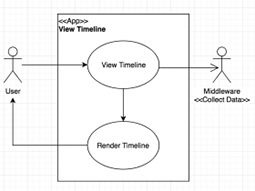
\includegraphics[]{view-timeline.png}  
\caption{\small \sl Use case diagram of a user view his own timeline. \label{fig:data_collect_user}}  
\end{center}  
\end{figure}

\begin{lstlisting}[caption=Hybrid-Metrics.js Example]
import React from 'react';
import Display from './Display';
import collect from 'hybrid-metrics';
import './App.css';

class App extends React.Component {
  view_timeline() {
    collect('view_timeline')
    timeline = Display.Timeline(user_id) 
    return { 
      timeline
    }
  } 
}
export default App;
\end{lstlisting}

Figure 2 shows a use case diagram of a user using an application and changing the background image. The new image information and the save new background image information is sent to the web service.

Listing 1 shows an example of what the middleware looks like when implemented in an application. In this example the middleware is used to collect user interaction information when the user views his own timeline. The framework allows the developer to identify a class, method, or function. The framework then collects the information and stores it in an object. The middleware runs on a timed cycle and at the end of the cycle period the metrics are transmitted to the API endpoint. In addition to the name of the function that was hit the number of times the function was used is also collected. 

\begin{figure*}
  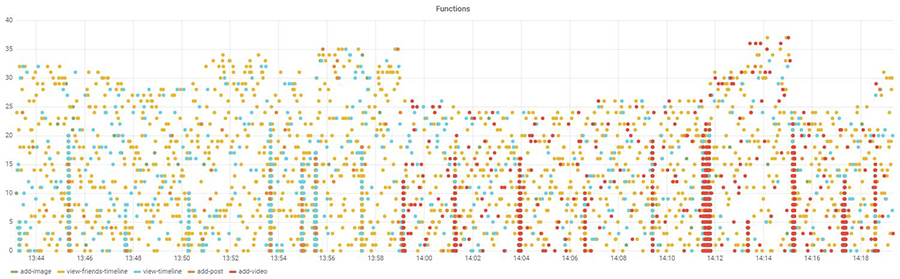
\includegraphics[width=\textwidth,height=4cm]{images/nf1_smaller.jpg}
  \caption{\small \sl Metrics Shows New Feature Adaptation\label{fig:new_feature_example}}  
\end{figure*}
\subsection{Web Service}
The web service is a nodejs application built using express.js. The web service provides an API that the middleware Nodejs module communicates with. We chose to use Node.js because it provides a lightweight web server which provides the required functionality. In In addition to providing the lightweight web server it is also written in JavaScript so it made life easier when transitioning between development for the web service and the Node module. 

\subsubsection{Application Programming Interface}
The API which the web service provides utilizes RESTful endpoints. When the middleware makes a POST call to the web service the web services parses the request. There are a couple of required fields for the request to be valid. The first required field is the name of the function that was called. The second is the number of times the function was called since the last time metrics were pushed to the API.

\subsubsection{Database Backend}
To handle the developer and application management aspects of the project we chose to use a the MySQL relational database. The MySQL database stores all of the information about developers and applications. It was an easy choice to pick a relational database for this purpose because the data is relational. We picked MySQL because it is well tested and we were familiar with it. 
 
Additionally, we also use MySQL as the database backend for metric collection. MySQL provides timestamps for each database entry. This timestamp allows us to compare values over a set period of time. Other databases provide this functionality as well but because we were already using it for the application management we decided to use it for this purpose as well. 

\subsection{Metric Analytics and Visualization}
The developer is able to view all collected metrics through a graphical user interface. The developer is able to query the database for different analytics. We showcase the metric analytics and visualization during the case study. Grafana provides graphs and time-series analysis UI elements such as bar charts, line charts, dots, and heat maps. Grafana helps to make the information that comes from the middleware more understandable and actionable for the developer. Grafana is also open source and integrates with a number of different data providers and databases which makes it perfect for future work.

\section{Developer Survey}
We surveyed 34 developers at local software engineering companies. We asked 20 questions which focused on how the developers felt about collecting user metrics, how important they felt understanding user behavior was, and if they had concerns about privacy while collecting metrics. Overall, the findings are conclusive. Developers care about collecting metrics, they would prioritize maintenance projects based on function usage, and they aren’t overly concerned with privacy issues while collecting the metrics. 

\subsection{Survey Bias}
The survey pool may have bias views towards the survey and the questions. The developers surveyed all have backgrounds as Department of Defense contractors. Most of the developers who responded all work at one company. 

\subsection{Findings}
Out of the 34 developers surveyed we found the following:
\begin{itemize}
  \item 61.8 percent of developers think user metric collection is important 
  \item 76.5 percent believe it is important to know how often features of an application are used
  \item 88 percent of developers want to maximize time when maintaining existing applications 
  \item 83.2 percent want to know how users use an application
  \item 79.4 percent would prioritize work based on user behavior. 
  \item 85.3 percent of developers are not concerned about user privacy while collecting usage metrics
\end{itemize}
This survey answers our first question. 83.2 percent of developers surveyed would find user behavior metrics useful. 79.4 percent would prioritize work based on the user behavior metrics.

\section{Case Study}
In order to showcase the benefits of the framework and middleware we conducted a simulated case study using a custom python script which sent simulated metrics at set intervals to the API service. 

\subsection{Study Operations}
\begin{lstlisting}[caption=sim.py Example][language=Python]
user_feature_weights = {
  "add-image": 1,
  "add-post": 1,
  "view-timeline": 24,
  "view-friends-timeline": 24,
}
for feature, weight in user_feature_weights.items():
  for x in xrange(randint(0, weight)):
    user_features.append(feature)
    
\end{lstlisting}
The study took a simple mobile application which was modeled after a social media application with four core functions. The functions are view-timeline, view-friends-timeline, add-post, and add-image. After collecting metrics for a period of time we introduce a new creator function called add-video. Based on the data gathered from the empirical study we are able to conclude that the framework and middleware provide insights that help developers maximize their resources and monitor user adaptation for new features.

The features were broken out into two categories, creator and consumer. Creators make up a small percentage, around 3 percent, of users compared to the consumers. Based on this information our simulation weighted the consumer functions over the creator functions with a ratio of 1 to 25.

We made 200 simulated users and loop over the users every second. These users are then randomly assigned a function out of the user-features array which we populated based on the weights of each function. After they are assigned a random feature they are then assigned a random number of usages ranging from 0 to 50. We provide a usage number because the middleware collects metrics and usage numbers for five minutes before pushing the metrics to the API. As the simulation loops the time to post to the API is randomized as well. We randomize the time to post to better model user behavior. We did not want all of the API requests to come in at precisely one second intervals.

\subsection{Results and Analysis}
\begin{figure}  
\begin{center}  
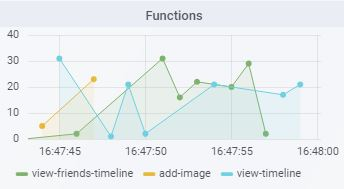
\includegraphics[]{freq.JPG}  
\caption{\small \sl Frequency of Usage\label{fig:freq_example}}  
\end{center}  
\end{figure}  
We were able to collect metrics from the case study and identify user trends. We were able to see user behavior metrics in the form of function usage. The consumer functions, view timeline and view friends timeline were the most popular features of our simulated application. The creator functions were used but not as heavily. 

Figure 3 shows an example of the metrics UI where we highlight the point which we add a new feature to the application. The new feature, add-video, had high user adoption and we can see that from the metrics collected. This answers the second evaluation question, we are able to identify user behavior from the application.

Figure 4 shows an example of the Grafana UI where we are able to tell how often a function is used over a period of time. Looking at this example we can see the view-friends-timeline and view-timeline are used much more frequently than add-image. This makes sense because consumer functions are used more often than creator functions. This figure answers the fourth evaluation question, we are able to identify function frequency use. 

The case study helped us answer two of the evaluation questions. It showed us that the application is able to identify user behaviors. It also showed that we are able to identify frequency of function usage.

\section{Discussion}
The application provided some interesting insights. The first insight was that we were able to identify user adaptation of a new feature. Figure 3 shows a very clear delineation of when a new feature came online. We can also see that it was a popular feature based on the amount of usage it received. This information could be very valuable to a developer to understand the scope of feature adaptation. We were also able to identify the frequency of function usage across a period of time. This information could potentially help a developer know where to focus testing, development, forecast resources, and identify possible bugs. 

The responses from the survey were interesting. We have attached the survey results for all of the questions to this paper. The most surprising response for us was that developers are not concerned about user privacy while collecting metrics. In today’s age of information sensitivity and privacy concerns we would have thought more developers would be concerned. We were happy that the survey data reinforced what we believed. Developer want to know how their applications are being used and that they would prioritize work based on such metrics. 

\section{Threats to Validity}
The first threat to the validity of the case study is that it was a simulation. We made a number of assumptions throughout the simulation as well.  The first assumption we made was that creator functions would make up about 3 percent of the functions called. This assumption was made based on research that was taken from social media web site statistics. We could not find good statistical information regarding mobile application usage and the difference between creators and consumers. 

The second assumption we made was that mobile devices would always have internet connectivity and that content would be uploaded every minute. We made this assumption to keep our simulation simple. This assumption did not impact any of the functionality of the middleware but may have skewed the way the metrics present in the time-series analysis graphs.

The third assumption we made was that the add-video function would be popular. We made this assumption for the sake of the simulation to show what a popular feature would look like had one been added to an existing application that was already monitored using our middleware. 

\section{Related Work}
Wu et. all ~\cite{appcheck}, wrote about a testing service for android using crowd sourcing. They used a web client to get mobile applications in front of users. The primary focus of the crowd-source testing was user interaction with the UI using metrics from clicks, long clicks, typing, scrolling, and pinching. Wu et all even have a replay feature to see how the user interacted with the UI. 

Ferreira et all  ~\cite{aware}, have developed a framework title AWARE. Their research focuses on mobile context for capturing, inferring, and generating context on mobile devices.  They accomplish this by collecting details of sensor data and uploading the data to a cloud. Their research is similar in that they have a client server framework and are collecting user metrics and pushing the data to a server. Their research is focused on understanding what a user is doing based on sensor data and then use that information to execute some intent in the application.

There are also tools that exist that are excellent at collecting hardware metrics from mobile applications. One such tool is app metrics from IBM which provides insights into the operating environment, CPU utilization, memory usage, and database queries ~\cite{ibm-appmetrics}.

New Relic is an application performance monitoring and management tool. New Relic provides a suite of tools to help developers monitor and improve their applications. The suite offers tools that measure response times, throughput, and error rates. In addition New Relic can be used to monitor thread profiles, transaction metrics, and key business transactions. New Relic is primary used to monitor web applications but it can be used to monitor applications built using PhoneGap which utilize HTML 5 web views for user graphical interfaces. The research presented in this paper and the user interaction metrics collected from the framework are different from New Relic because the metrics collected from the mobile applications are at the code level. We can track and understand user interactions at the function level. New Relic sits on top of an existing application but it does not tie in to the code the way our framework does. Since our framework integrates at such a low level we are able to collect metrics that are specific to user interactions ~\cite{newrelic}.

Google Analytics is another application that provides insights to performance and application management. Google Analytics is a powerful analytics platform that developers use to gather metrics such as the number of users using an application, what actions the users are taking, measure in-app payments, and visualize user navigation path ~\cite{googleAnalytics}. Google Analytics, like New Relic, was first developed for use in web sites and web applications. Google now offers Analytics for use with mobile applications. Google Analytics is similar to our framework in that you can glean information about user activity from the platform. Our framework is different from Google Analytics because we are able to gather the data that is passed from one function to another. This allows us to look directly at the user\'s interaction with the application to understand better how the application is utilized.


\section{Conclusion}
It is important for developers to understand how their applications are being used so that they can prioritize development, testing, and maintenance of new features. We have presented an approach to collect user interaction metrics from hybrid mobile applications which give insights that will help developer understand user interactions. Through this research have contributed an opensource middleware, a RESTful web API service, a developer survey, and discussion on our approach. Overall, we were able to answer all of our evaluation questions. We were also able to, through the survey, show that such a tool which provides these metrics would be useful to developers.

\section{Future Work}
The framework along with the time series analysis can be used to measure and identify usage trends in any web-based application. Some future work examples that we would like to explore would be identifying bugs based on user interactions. We could do this several ways and possibly build off of existing research which leverages time series analysis such as Coker et all ~\cite{bdbugs} research where they developed a method using time series analysis to prioritize bugs. Although our research does not touch on prioritization or on identifying bugs our framework could be used to identify usage trends that may highlight bugs within the application.

Another area would be to take measurements of the impact of the middleware on real world software examples. It would be interesting to measure the code growth and the resource utilization of an exiting application with before and after metrics. 

An additional area of opportunity would be to use the API service with standard mobile applications. The middleware would be reasonably easy to develop for native Android or iOS applications. 

The web service needs to be hardened against malicious users. It also needs to support multiple developers in separate Grafana UIs. One avenue we could go to improve both issues is to implement a token-based approach for the web UI endpoint. If the UI endpoint receives metrics, then it will first look for a developer token. If the token is valid then it will tag the metrics with the developer’s ID and post the information to the database. This would improve the system against malicious users who may just want to provide false information by keeping out the false information. This would also allow the system to support multiple users. We could query first by developer ID and then by features or function names. 